\documentclass[10pt,a4paper]{amsart}
\usepackage[margin=19mm]{geometry}
\usepackage{amsmath,amssymb,mathtools}
\usepackage[scr=rsfs,cal=euler]{mathalfa}
\usepackage{xfrac}
\usepackage[unicode,hidelinks,bookmarks=false]{hyperref}
\newcommand{\ie}{i.e.\ }
\newcommand{\cf}{cf.\ }
\newcommand{\resp}{respectively\ }
\newcommand{\Subsection}{\subsection}
\providecommand{\nobreakdash}{\nobreak\hbox{-}}
\setlength{\emergencystretch}{2em}
\multlinegap0pt
\usepackage{tikz}
\usepackage{caption}
\usepackage{amssymb}
\usepackage{xcolor}
\newtheorem{proposition}{Proposition}
\newtheorem{lemma}{Lemma}
\newtheorem{scope}{Scope}
\title{Remarks on the relative isoperimetric profile of polygonal domains in $\mathbb{R}^2$}
\author{Jason DeVito, Robert DeYeso III, Ezra Nance, Robert Niedzialomski}
\date{Source: arXiv:2605.23149v1 (CC BY 4.0)}
\begin{document}
\maketitle

\noindent\emph{Source and licence.} Remarks on the relative isoperimetric profile of polygonal domains in $\mathbb{R}^2$. Version arXiv:2605.23149v1 (CC BY 4.0), distributed by arXiv under the Creative Commons Attribution 4.0 International licence, http://creativecommons.org/licenses/by/4.0/, as recorded in the arXiv licence metadata for this exact version and shown on the abstract page https://arxiv.org/abs/2605.23149v1. Full licence notice: \texttt{licenses/arxiv-2605.23149-CC-BY-4.0.txt}.\par\smallskip

\noindent\textit{Editorial scope.} Counted unit: the article's proposition prop:convexcorner (source0.tex lines 249--256). The article's complete original proof of it is delivered with it (source0.tex lines 258--366, one \texttt{proof} environment of 109 lines). No mathematics is written, repaired or re-derived: the statement and the proof are the article's own lines, in the article's own notation, and no retained line is substituted or re-flowed.  Retained uncounted as the source-local context the proof needs: lines 200--201; lines 235--236.  Nothing was omitted from any retained span, so the package carries no omission record.  No retained line contains a citation, so the wrapper carries no bibliography and no bibliography entry.  The retained lines contain the article's own diagram code, which the wrapper typesets with the standard tikz packages; no image file is delivered and the package declares no asset dependency.  Editorial formatting only, in addition: an AMS \texttt{amsart} preamble that restates the article's own declarations and macros used by the retained lines, namely the environments \texttt{proposition}, \texttt{lemma}, \texttt{scope} on separate counters, together with the standard packages those lines need.  The retained environments print in this document as Proposition 1, Lemma 1, Scope 1 in order of appearance, whereas the article prints the same items with the numbering of its own full document.  The complete native source of the article as distributed in the arXiv e-print for this exact version is bundled unchanged as \texttt{sources/201187/source0.tex}.
\begin{proposition}\label{prop:circleTangentToSide} Let $Q\subseteq\mathbb{R}^2$ be a polygonal region and let $K\in Q$ be a convex corner.  Suppose that $S\subseteq Q$ has a unique smooth component containing $K$.  If this component is tangent to $Q$ at $K$, then $S$ is not an isoperimetric minimizer.
\end{proposition}

\begin{lemma}\label{lem:chordAreaOrder}Suppose $C$ is a circle of radius $r$.  Then the smaller area determined by a chord of length $\ell$ has area  $O(\ell^3)$.
\end{lemma}

\begin{proposition}\label{prop:convexcorner}Suppose $Q\subseteq\mathbb{R}^2$ is a polygonal region and $K\in Q$ is a convex corner.  Suppose $S\subseteq Q$ and $\partial S$ contains exactly one smooth component containing $K$, which is either a line segment or an arc of a circle.  Then there exists $S' \subseteq Q$, an arbitrarily small deformation of $S$, with the following properties:

\begin{itemize}\item $|S| = |S'|$
\item $P(S) > P(S')$
\item No smooth component of $\partial S'$ contains $K$.
\end{itemize}

\end{proposition}

\begin{proof}
    We will first consider the case when the smooth boundary component containing $K$ is a line segment. For a small enough neighborhood of $K$, we can consider only the corner and this single line segment. Let $P$ be a point on $\partial S$ and let $\ell$ be the length of this line. Note that since $K$ is a convex corner, $\partial S$ makes at least one acute angle with $\partial Q$. Thus, without loss of generality, we have the following picture for a neighborhood of $K$.

    \begin{center}
        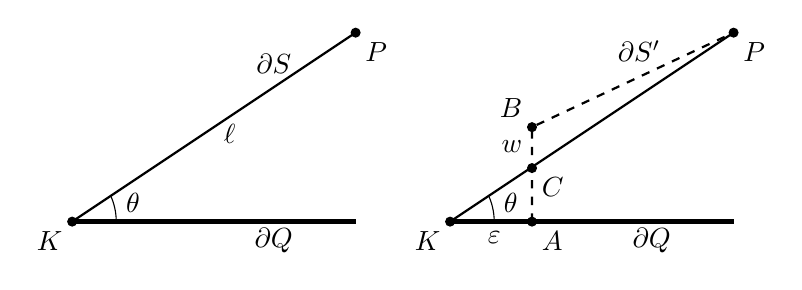
\begin{tikzpicture}[scale=0.8]
            \draw[ultra thick] (-4.5,2) -- (0,2);
            \draw[thick] (-4.5,2) -- (0,5);
            \filldraw (-4.5,2) circle (2pt) node[anchor=north east] {$K$};
            \draw (-2,3.4) node {$\ell$};
            \draw (-1.3,4.5) node {$\partial S$};
            \draw (-1.3,1.7) node {$\partial Q$};
            %\draw[thick] (-4.5,2) arc (156.4:91:5);
            \draw (-3.8,2) arc (0:25:1);
            \draw (-3.8,2.3) node[anchor=west] {$\theta$};
            \filldraw (0,5) circle (2pt) node[anchor=north west] {$P$};
            \begin{scope}[shift={(6,0)}]
                \draw[ultra thick] (-4.5,2) -- (0,2);
                \draw[thick] (-4.5,2) -- (0,5);
                \filldraw (-4.5,2) circle (2pt) node[anchor=north east] {$K$};
                \filldraw (-3.2,2) circle (2pt) node[anchor=north west] {$A$};
                \filldraw (-3.2,3.5) circle (2pt) node[anchor=south east] {$B$};
                \draw (-3.8,2) node[anchor=north] {$\varepsilon$};
                %\draw (-2,3.4) node {$\ell$};
                \draw (-3.2,3.2) node[anchor=east] {$w$};
                \draw (-1.5,4.7) node {$\partial S'$};
                \draw (-1.3,1.7) node {$\partial Q$};
                \draw (-3.8,2) arc (0:25:1);
                \draw (-3.8,2.3) node[anchor=west] {$\theta$};
                \filldraw (0,5) circle (2pt) node[anchor=north west] {$P$};
                \draw[thick,dashed] (-3.2,2) -- (-3.2, 3.5) -- (0,5);
                \filldraw (-3.2,2.85) circle (2pt) node[anchor=north west] {$C$};
            \end{scope}
        \end{tikzpicture}
        \captionof{figure}{On the left we have $\partial S$ intersecting a corner $K$. On the right we have a deformation $\partial S'$ which avoids corner $K$.}\label{fig:deformAwayFromCorner}
    \end{center}

    We will now deform $\partial S$ to $\partial S'$ with the desired properties. Consider a point $A$ which is $\varepsilon$ units away from the corner, and let $B$ be the point directly above $A$ so that $|S| = |S'|$. Let $C$ be the intersection point of $\overline{KP}$ and $\overline{AB}$, and let $w$ be the length of $\overline{BC}$. Note that in order for $|S| = |S'|$, we need the triangles $\Delta ACK$ and $\Delta BCP$ to have the same area. In other words, we need $$\frac{1}{2}\varepsilon^2 \tan\theta = \frac{1}{2}(\ell - \varepsilon\sec\theta)w\cos\theta.$$ This is true when
    \[
        w = \frac{\varepsilon^2\tan\theta}{\ell\cos\theta - \varepsilon}.
    \]
    Having achieved that $|S| = |S'|$, we now compare perimeters of the boundaries.  Note that $P(S) > P(S')$ if and only if $\left|\,\overline{KP}\,\right| > \left|\,\overline{AB}\,\right| + \left|\,\overline{BP}\,\right|.$
    As $|\overline{KP}|  = |\overline{KC}| + |\overline{CP}|$, it follows from the triangle inequality that this inequality is true if
    \begin{equation}\label{eq:lowerPerim}
        \left|\,\overline{KC}\,\right| > 
        2\left|\,\overline{BC}\,\right| + 
        \left|\,\overline{AC}\,\right|.
    \end{equation}
    Indeed, \begin{align*} |\overline{KP}| &= |\overline{KC}|+|\overline{PC}|\\
    & > 2|\overline{BC}| +|\overline{AC}| + |\overline{PC}|\\
    &= (|\overline{BC}| + |\overline{AC}|) + (|\overline{BC}| + |\overline{PC}|)\\
    & \geq |\overline{AB}| + |\overline{BP}|.\end{align*}
    
    Substituting into inequality \eqref{eq:lowerPerim} and rearranging, we find that inequality \eqref{eq:lowerPerim} holds if and only if 
    \begin{equation}\label{eq:lowerPerim2}
        2\varepsilon^2\tan\theta < \varepsilon(\ell - \varepsilon\sec\theta)(1-\sin\theta).
    \end{equation}
    Notice that since $\theta \in (0,\tfrac{\pi}{2})$, all factors in (\ref{eq:lowerPerim2}) are positive.  In addition, the left side is $O(\varepsilon^2)$ while the right side is $O(\varepsilon)$.  It follows that for all sufficiently small $\varepsilon$, the inequality \eqref{eq:lowerPerim2} holds. Hence, the proof is complete in the case where the smooth boundary component of $\partial S$ is a line segment.

    Now we will consider the case when the smooth boundary component containing $K$ is the an of a circle. By Proposition \ref{prop:circleTangentToSide}, we can assume that $\partial S$ does not touch $K$ tangentially to $Q$. Furthermore, since $K$ is a convex corner, $\partial S$ makes an acute angle at $K$ with at least one side of $\partial Q$. Thus, without loss of generality, we can assume that we have a neighborhood of $K$ which looks like one of the following, depending on the curvature.

    \begin{center}
        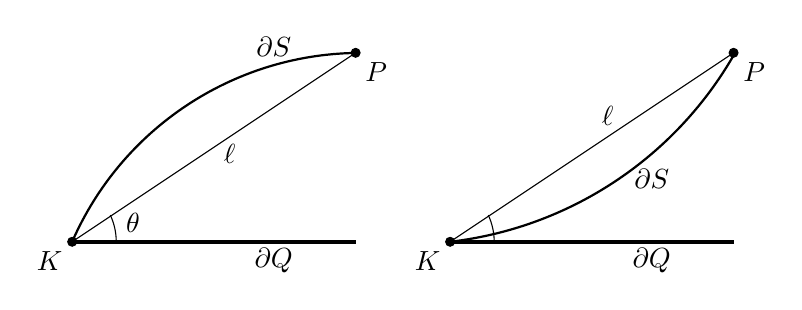
\begin{tikzpicture}[scale=0.8]
            \draw[ultra thick] (-4.5,2) -- (0,2);
            \draw (-4.5,2) -- (0,5);
            \filldraw (-4.5,2) circle (2pt) node[anchor=north east] {$K$};
            \draw (-2,3.4) node {$\ell$};
            \draw (-1.3,5.1) node {$\partial S$};
            \draw (-1.3,1.7) node {$\partial Q$};
            \draw[thick] (-4.5,2) arc (156.4:91:5);
            \draw (-3.8,2) arc (0:25:1);
            \draw (-3.8,2.3) node[anchor=west] {$\theta$};
            \filldraw (0,5) circle (2pt) node[anchor=north west] {$P$};
        \begin{scope}[shift={(6,0)}]
            \draw[ultra thick] (-4.5,2) -- (0,2);
            \draw (-4.5,2) -- (0,5);
            \filldraw (-4.5,2) circle (2pt) node[anchor=north east] {$K$};
            \draw (-2,4) node {$\ell$};
            \draw (-1.3,3) node {$\partial S$};
            \draw (-1.3,1.7) node {$\partial Q$};
            \draw[thick] (-4.5,2) arc (-83.34:-30:6);
            \draw (-3.8,2) arc (0:25:1);
            \filldraw (0,5) circle (2pt) node[anchor=north west] {$P$};
        \end{scope}
        \end{tikzpicture}
        \captionof{figure}{Both possibilities for a circular arc to touch a corner acutely.}\label{fig:arcTouchingCorner}
    \end{center}
    
    Consider a point $P \in \partial S$, and let $\ell$ be the length of the secant line $\overline{KP}$. Now we can repeat the argument for the straight line case to create $\partial S'$ away from corner $K$. The only difference is that now $w$ will have to take into account the area, say $\delta$, between $\partial S$ and the secant line $\overline{KP}$. By doing this we can ensure that $|S| = |S'|$. Following the same logic as before, we will have that $P(S) > P(S')$ if
    \begin{equation}\label{eq:lowerPerim3}
        2\varepsilon^2\tan\theta  \pm \delta < \varepsilon(\ell - \varepsilon\sec\theta)(1-\sin\theta).
    \end{equation}
    Let $\varepsilon = \lambda \ell$. By Lemma \ref{lem:chordAreaOrder}, $\delta = O(\ell^3)$. Therefore, inequality \eqref{eq:lowerPerim3} is true if and only if there exists some $\lambda \in (0,1)$ and some $\ell > 0$ such that
    \[
        2\lambda^2\ell^2\tan\theta  \pm O(\ell^3) < \lambda\ell^2(1 - \lambda\sec\theta)(1-\sin\theta).
    \]
    We divide by $\ell^2$ and rearrange to see that inequality \eqref{eq:lowerPerim3} is true if and only if
    \[
        O(\ell) < \lambda(1-\sin\theta) - \lambda^2\sec\theta(1+\sin\theta).
    \]
    Let $\theta_{1}$ be the larger of the two angles formed by the tangent line at $K$ and the secant line at $K$. Then
    \[
        \lambda(1-\sin\theta_{1}) - \lambda^2\sec\theta_{1}(1+\sin\theta_{1}) < \lambda(1-\sin\theta) - \lambda^2\sec\theta(1+\sin\theta)
    \]
 for any $0\leq \theta < \theta_1$.   Thus, we have $P(S) > P(S')$ if
    \[
        O(\ell) < \lambda(1-\sin\theta_{1}) - \lambda^2\sec\theta_{1}(1+\sin\theta_{1}).
    \]
    We can choose $\lambda \in (0,1)$ so that the right-hand side is positive. Also, since the right-hand side is independent of $\ell$, we can then shrink $\ell$ to achieve our result. The circular arc case is done.
\end{proof}

\end{document}
